\subsection{Error Pattern Assessment}
\label{sec:error_pattern_assessment}
\label{sec:error_pattern}

\begin{figure*}[htbp]
\centering
\subfigure[Single-Domain Face Biometrics]{\label{fig:4a}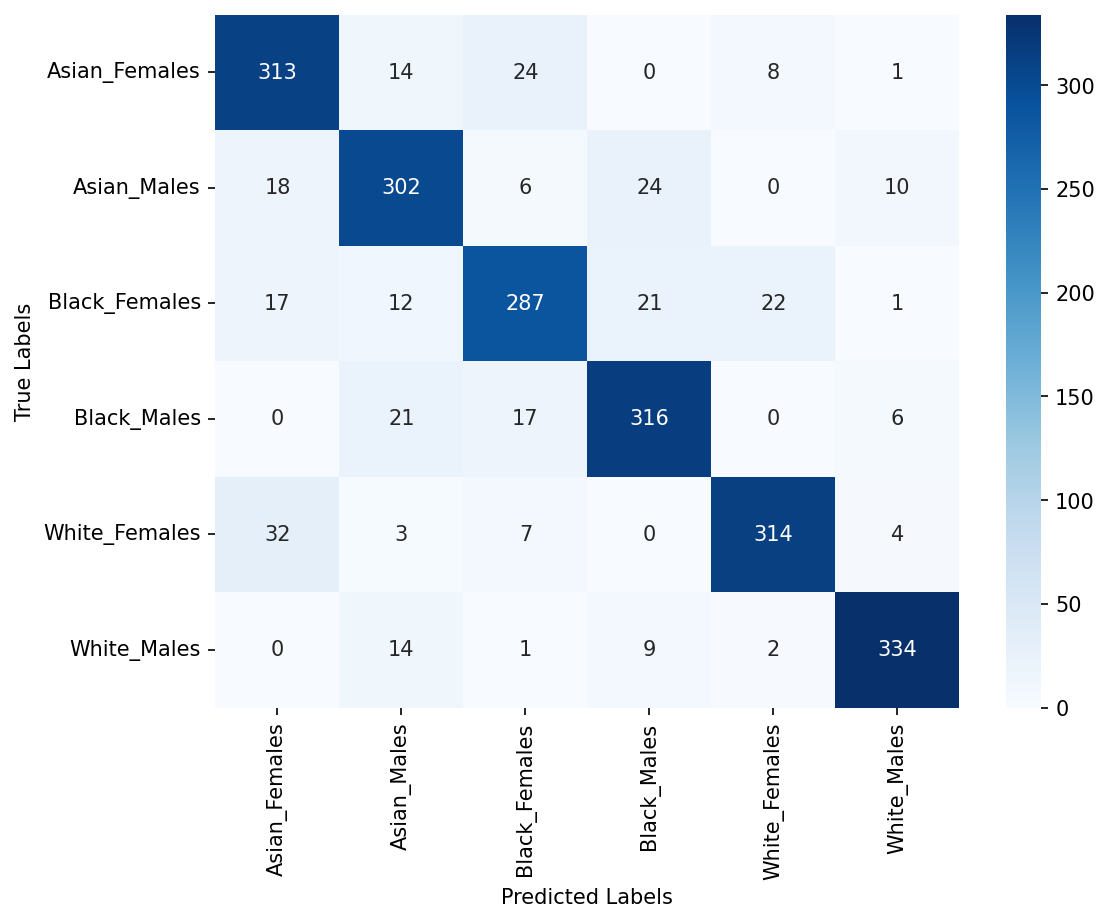
\includegraphics[width=0.32\textwidth]{confusion_matrix_lr_single_v1.1.png}}\hfill%
\subfigure[Dual-Domain Emotion $\oplus$ Face]{\label{fig:4b}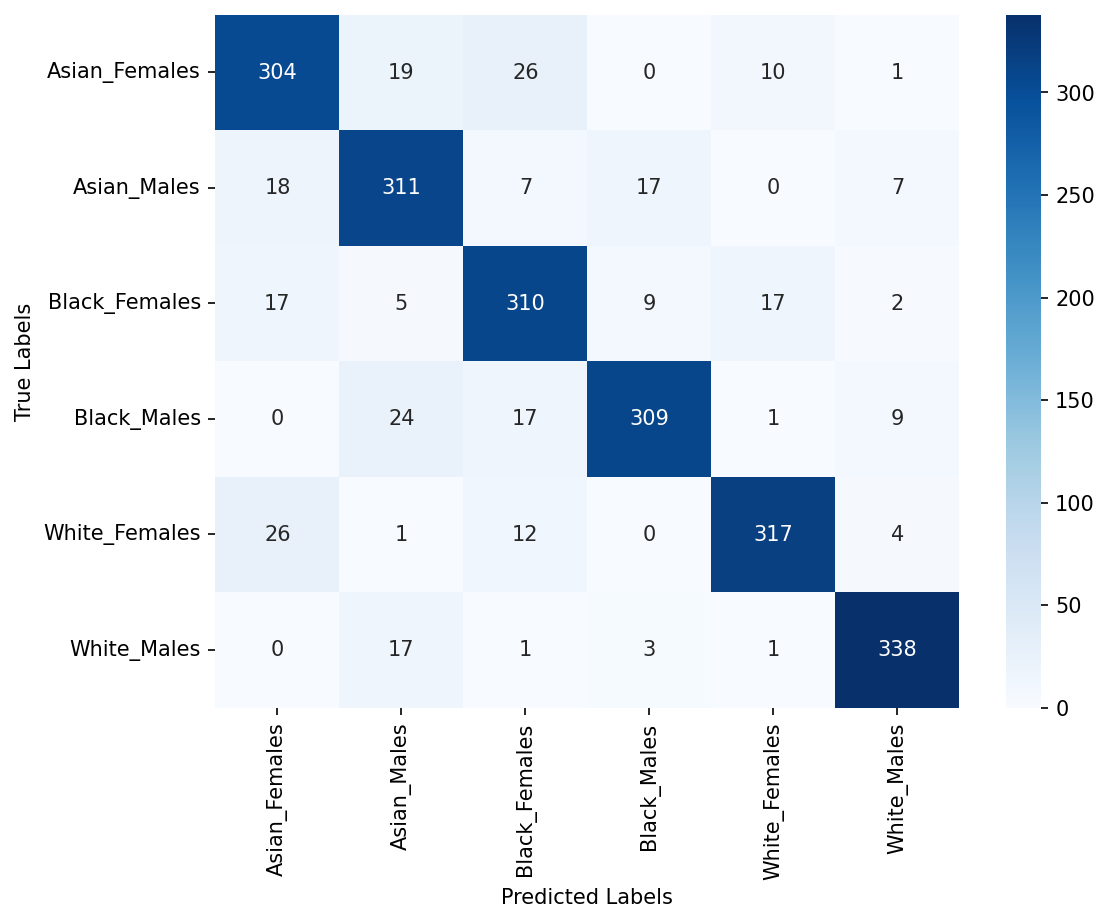
\includegraphics[width=0.32\textwidth]{confusion_matrix_lr_dual_v1.1.png}}\hfill%
\subfigure[Tri-Domain Face $\oplus$ Emotion $\oplus$ Age]{\label{fig:4c}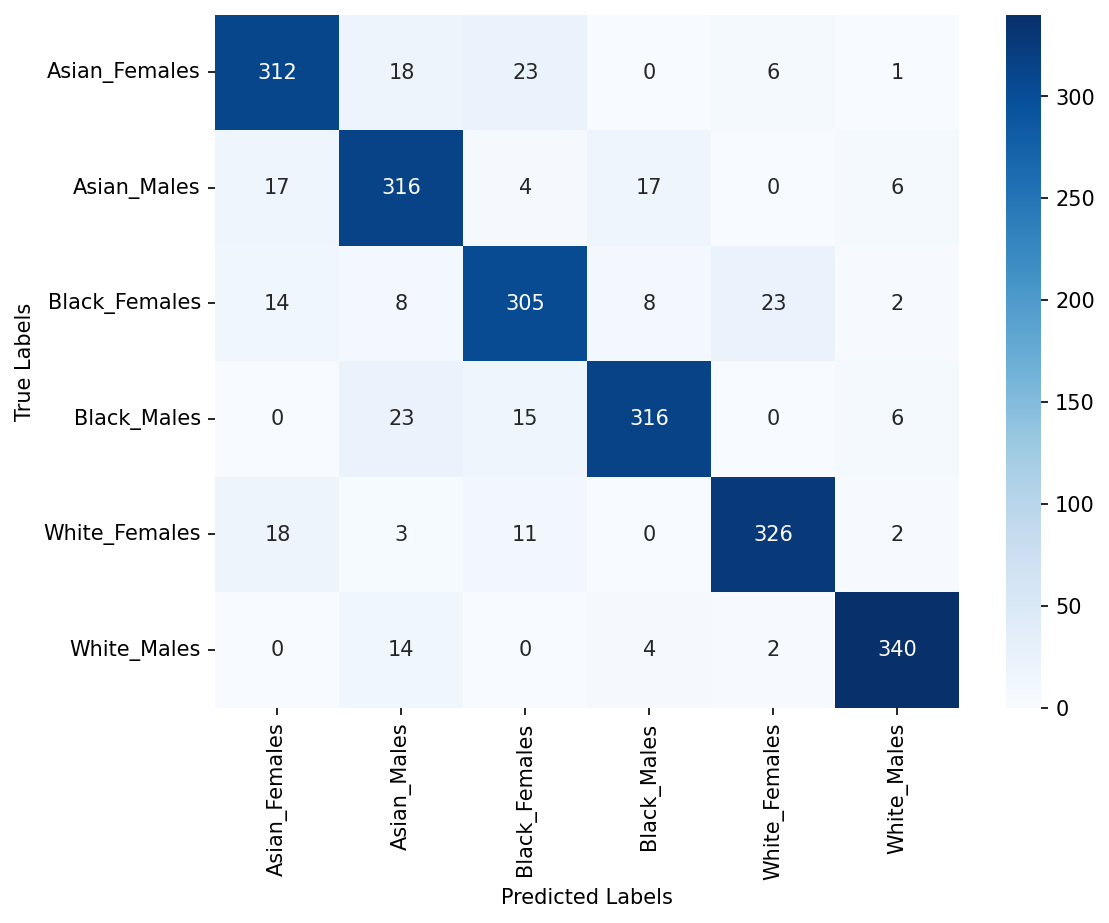
\includegraphics[width=0.32\textwidth]{confusion_matrix_lr_tri_v1.1.png}}
\caption{Comparative 6 $\times$ 6 Confusion Matrices of Logistic Regression on the Held-Out Subject-Disjoint Test Set: (a) Single-Domain Face Biometrics, (b) Dual-Domain Emotion $\oplus$ Face, and (c) Tri-Domain Face $\oplus$ Emotion $\oplus$ Age.}
\label{fig:4}
\label{fig:IV}
\end{figure*}

% Table 16: Placed here before paragraph 1 (Page 11) so it queues for Page 13 top
\begin{table*}[t]
\caption{Contextual and Controlled Comparison of the Proposed Framework on the DemogPairs Dataset.}
\label{tab:16}
\label{tab:XVI}
\centering
\footnotesize
\setlength{\tabcolsep}{6pt}
\resizebox{\textwidth}{!}{%
\begin{tabular}{lccccc}
\toprule
\textbf{Model} & \textbf{Data Split Protocol} & \textbf{Accuracy (\%)} & \textbf{Precision (\%)} & \textbf{Recall (\%)} & \textbf{F1-Score (\%)} \\
\midrule
MD-ViT + XGBoost~\cite{ref20} & Stratified & 89.07 & 89.12 & 89.07 & 89.01 \\
Dual-ViT + SVM~\cite{ref19} & Stratified & 92.41 & 92.48 & 92.41 & 92.38 \\
\textbf{Proposed Tri-Domain + SVM} & \textbf{Stratified} & \textbf{93.70} & \textbf{93.72} & \textbf{93.70} & \textbf{93.69} \\
\midrule
Single-Domain \textit{Face} + LR & Subject-Disjoint & 86.39 & 86.46 & 86.39 & 86.40 \\
Single-Domain \textit{Face} + SVM & Subject-Disjoint & 86.16 & 86.24 & 86.16 & 86.19 \\
Single-Domain \textit{Emotion} + SVM & Subject-Disjoint & 85.79 & 85.84 & 85.79 & 85.80 \\
Single-Domain \textit{Age} + SVM & Subject-Disjoint & 82.55 & 82.68 & 82.55 & 82.58 \\
Dual-Domain \textit{Emotion} $\oplus$ \textit{Face} + SVM & Subject-Disjoint & 88.43 & 88.50 & 88.43 & 88.44 \\
Tri-Domain + RF & Subject-Disjoint & 85.00 & 85.06 & 85.00 & 84.93 \\
Dual-Domain \textit{Emotion} $\oplus$ \textit{Face} + GNB & Subject-Disjoint & 84.31 & 84.37 & 84.31 & 84.30 \\
Proposed Tri-Domain + SVM & Subject-Disjoint & 88.61 & 88.71 & 88.61 & 88.63 \\
\textbf{Proposed Tri-Domain + LR} & \textbf{Subject-Disjoint} & \textbf{88.66} & \textbf{88.75} & \textbf{88.66} & \textbf{88.68} \\
\bottomrule
\end{tabular}%
}
\end{table*}

The dynamics of classification error reduction in the LR model are evaluated across three stages of representation fusion schemes on the held-out subject-disjoint test set via 6 $\times$ 6 confusion matrices as presented in Figure~\ref{fig:4}. Empirical evaluation demonstrates a consistent cumulative error reduction as the latent representation domains expand. The single-domain Face baseline model produces 294 prediction errors with an accuracy of 86.39\%. The integration of affective representations in the dual-domain Emotion $\oplus$ Face configuration reduces the number of misclassifications to 271 samples (87.45\% accuracy). The addition of biological aging morphological features in the tri-domain Face $\oplus$ Emotion $\oplus$ Age scheme successfully reduces errors to its lowest point of 245 samples with an accuracy of 88.66\%. This stepwise reduction pattern demonstrates the complementary advantage of multi-domain fusion in sharpening separation margins across demographic subgroups.

Quantitative decomposition of the off-diagonal cells in the confusion matrices reveals that the classification error pattern is dominated by same-gender cross-race misclassifications. In the tri-domain model (245 errors), intra-gender cross-race confusion accounts for 165 images (67.35\% of total errors or 7.64\% of all test samples), declining significantly from 194 cases in the single-domain model. The largest confusion cells are observed for Black Males to Asian Males (23 images), Black Females to White Females (23 images), and Asian Females to Black Females (23 images). Conversely, cross-gender errors amount to only 80 images (32.65\% of total errors or 3.70\% of all test samples). This pattern aligns with the recall profile of Black Females (84.72\%), where 37 of their 55 errors occur intra-gender toward White Females (23) and Asian Females (14).

The cross-race visual overlap phenomenon underlying this misclassification pattern is examined objectively based purely on the distribution of image visual variations, without introducing independently untested biological causal assumptions. Empirical evaluation shows that the confusion matrices reflect the observational data distribution characteristics within the evaluated corpus. The addition of biological aging representations provides a measurable contribution in suppressing intra-gender cross-race confusion from 185 to 165 cases, consistent with the statistical significance of McNemar's test ($p = 0.0073$). This qualification affirms that the superiority of multi-domain fusion originates from complementary latent feature covariate enrichment, thereby resolving visual ambiguities in the representation space without relying on phenotypic speculations or lighting conditions.
